\documentclass[a4paper,twoside]{article}

\usepackage{epsfig}
\usepackage{subcaption}
\usepackage{calc}
\usepackage{amssymb}
\usepackage{amstext}
\usepackage{amsmath}
\usepackage{amsthm}
\usepackage{multicol}
\usepackage{pslatex}
\usepackage{apalike}
\usepackage{SCITEPRESS}     % Please add other packages that you may need BEFORE the SCITEPRESS.sty package.


\begin{document}

\title{Authors' Instructions: Preparation of Camera-Ready Contributions to SCITEPRESS Proceedings}

\author{\authorname{First Author Name\sup{1}\orcidAuthor{0000-0000-0000-0000}, Second Author Name\sup{1}\orcidAuthor{0000-0000-0000-0000} and Third Author Name\sup{2}\orcidAuthor{0000-0000-0000-0000}}
\affiliation{\sup{1}Institute of Problem Solving, XYZ University, My Street, MyTown, MyCountry}
\affiliation{\sup{2}Department of Computing, Main University, MySecondTown, MyCountry}
\email{\{f\_author, s\_author\}@ips.xyz.edu, t\_author@dc.mu.edu}
}

\keywords{interactive, Spark, Kubernetes, YARN, cluster.}

\abstract{Various cloud providers offer integrated platforms for interactive development in notebooks for processing & analysis of Big Data on large compute clusters. Such platforms enable users to easily leverage frameworks like Apache Spark as well as manage cluster resources. However, Data Scientists & Engineers are faced with the lack of a similar holistic solution when working with on-premises infrastructure. Users are currently not able to profit from a central point of administration to access a notebooks’ UI, manage notebook kernels, allocate resources for frameworks like Apache Spark or monitor cluster workloads in general. To overcome these issues and provide on-premises users with a platform for interactive development, this paper proposes a cross-cluster architecture resulting from an extensive requirements engineering process. Based on open-source components, the designed platform provides an intuitive Web-UI that enables users to easily access notebooks, manage custom kernel-environments as well as monitor cluster resources and current workloads. Besides an admin panel for user restrictions, the platform provides isolation of user workloads and scalability by design.
The designed platform is evaluated against prior solutions for on-premises as well as from a user perspective by utilizing the User Experience Questionnaire, an independent benchmark tool for interactive products.}

\onecolumn \maketitle \normalsize \setcounter{footnote}{0} \vfill

\section{\uppercase{Introduction}}
\label{sec:introduction}

\begin{itemize}
    \item A lot of data available
    \item Efficient tools available (Spark, Notebooks, Resource Managers)
    \item These tools are complex
    \item Problem: On-Premises infrastructure is lacking in terms of out of the box solutions
    \item On-Premises are widely spread, especially in big companies
    \item Four companies, with above 250 000 employees were involved
    \item They have their own compute clusters
    \item They are missing a holistic platform for analytics on distributed data with Spark
    \item The Spark mode is restricted to client-mode from within an interactive environment, especially for solutions supporting on-premises infrastructure
\end{itemize}

\section{\uppercase{Foundations and related work}}

\begin{itemize}
    \item Spark as one of the main frameworks for distributed data
    \item Jupyter Notebooks becoming defacto standard for interactive analysis. 
    \item Various resource managers: Kubernetes, Hadoop YARN
    \item Various solutions are developed, Databricks (only for Cloud)
    \item or SWAN (proves, that CERN having own compute clusters had to implement an own solution)
\end{itemize}


\section{\uppercase{Requirements Engineering}}

On the one hand, since there are already a few platforms for interactive data science available, one has to analyze the current situation in order to find out, whether there is need for an additional platform claiming to outperform existing solutions in some aspects. To do so, one has to review existent solutions among users who work with distributed data on compute clusters and find a niche for such a product, proving there is indeed necessity for improvement. When considering the fact, that almost all existing platforms focus on a cloud-offering, it appears that a holistic platform for interactive development is missing for on-premises infrastructure. However, it is quite likely that users working with such infrastructure have implemented their own, custom, solutions. Those need to be analyzed and reviewed as well. In that way, one gets an overview of platforms or, more general, solutions, used for both cloud and on-premises compute clusters.

On the other hand, in order to design and implement any kind of software, it is crucial to know the requirements carried by the users. By reviewing existent solutions and analyzing users needs it is possible to specify which functionalities might be missing or provide room for improvement.

With requirements engineering it is possible to analyze current state of platforms for interactive analysis of distributed data. Further, it allows to gather requirements which will then provide the foundation for design and implementation of said platform.




\begin{itemize}


    \item Requirements engineering is an iterative process used from the very beginning in the software development
    \item Allows to analyse current situation
    \item Allows to specify requirements for a software product
    \item Should be used to find out, what users are currently working with for interactive data analytics
    \item What are the pros and cons of used solutions
    \item How important the on-premises infrastructure is
    \item Should allow to specify requirements for a holistic platform for interactive analytics on distributed data
\end{itemize}

\subsection{Target group}

The target group can provide useful information resulting in actual requirements. Participants need to have significant experience in either data science or engineering on compute clusters, especially in terms of distributed data. This means they should have worked or are working with a framework that supports distributed data analysis, e.g. Apache Spark, preferably on a cluster. Furthermore, using some kind of interactive component (e.g. notebooks included in a third party platform or custom made), in combination with frameworks like Spark, is important since it provides information about the solutions users are currently using and how satisfied they are with them.

Besides data scientists and engineers, participants experienced in cluster administration are also of great value, since they know the complexity and issues of deploying as well as managing distributed infrastructure including the software running on it. 

As one can see, the target group is small and it is important to actually reach these kind of users, otherwise false conclusions will lead to false requirements. Since the target group is specified, one can move on to the first step of RE, namely to requirements elicitation.

\begin{itemize}
    \item A very specific and highly skilled target group is needed
    \item Data scientists and engineers
    \item Cluster administrators
\end{itemize}

\subsection{Conduction}

In order to elicit needed information from participants, two methods were used: a questionnaire and an interview. While a questionnaire allows to reach more participants and thus gather statistically reliable data, the interviews provide an opportunity to discuss various aspects more deeply. Participants either took part in the questionnaire and/or the interview. 

To actually merge results, both methods follow the same structure by collecting general information about participants and their use-cases, continuing with a section about the infrastructure as well as the setup they use to work with in terms of interactively explore or analyize distributed data. Finally, various features, that align to already existing solutions, are given to be evaluated by the participants. 

In total, 19 participants contributed to the requirements engineering process. One may think that’s rather a small probe, however, as shown later, those 19 participants are highly skilled and experienced in terms of cluster computing and/or cluster administration, which is a desired requirement for the target group. The results of the questionnaire and the interviews are presented in next section.

\subsection{Results}

The first important result is the fact, that the target group is indeed achieved. As shown in fig. \ref{fig:self_rating}, the participants are highly skilled in terms of data science or data engineering on distributed resources. In terms of cluster administration, the average of 2.52 of 5 results from the fact, that participants have the tendency to be skilled in only one of both. Thus data scientists or engineers are majority. Experts for both subjects, however, are included. Furthermore, participants spend on average 68\% of their working week dealing with compute clusters, which makes them even more reliable as an information source. 

\begin{figure}[!h]
  \centering
   {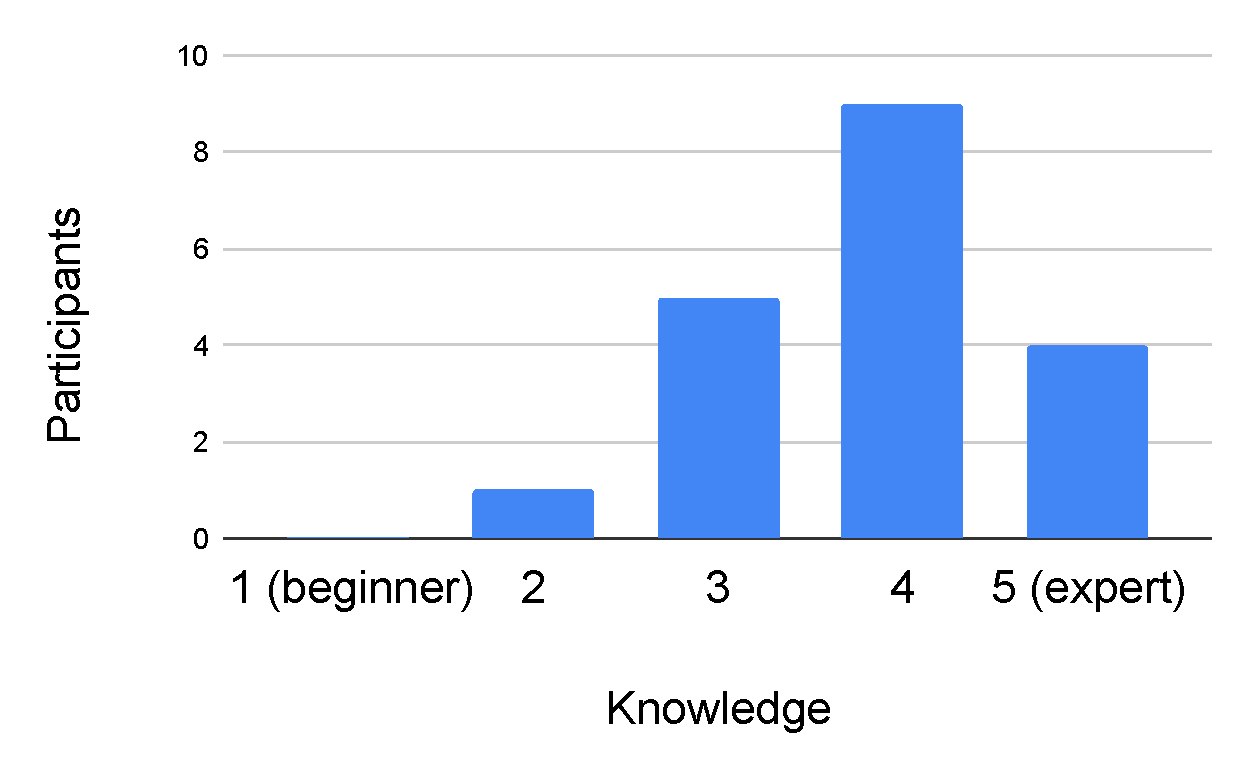
\epsfig{file = figs/rating_data_science.pdf, width = 5.5cm}}
  \caption{\textit{How would you rate your knowledge of data science / engineering in terms of distributed cluster computing?} On average 3.84 out of 5.}
  \label{fig:self_rating}
 \end{figure}

A big advantage is also the variance of industry sectors represented by the participants, with Retail (25\%) being the leading, but also automotive, finance, internet industry and three others. In terms of use-cases, batch processing (ETL) is by far the most frequent one (78\%). Further significant tasks are e.g. data streaming (53\%), software development (47\%) or machine learning (36\%). 

As one can see, compute clusters are present in various industry sectors and are used to solve numerous problems. Those problems have one thing in common, they all deal with data. The conducted survey and interviews show that users working with compute clusters mostly work with data in size between 100GB and 1000GB (31.7\%), however, datasets of above 1000GB are not uncommon (15.8\%). Comparing cloud and on-premises clusters, the total
percentage of users working with data above 1000GB is slightly higher for on-premises, namely 18\% versus 12\% for cloud.

\subsubsection{Infrastructure and general setup}

One of the fundamental discoveries of the requirements engineering process is the fact, that the on-premises infrastructure is widely represented. As shown in fig. \ref{fig:on_prem_vs_cloud}, on-premises infrastructure, with 58\%, is more popular among participants than cloud. Especially big companies tend to have their own compute clusters. 

\begin{figure}[!h]
  \centering
   {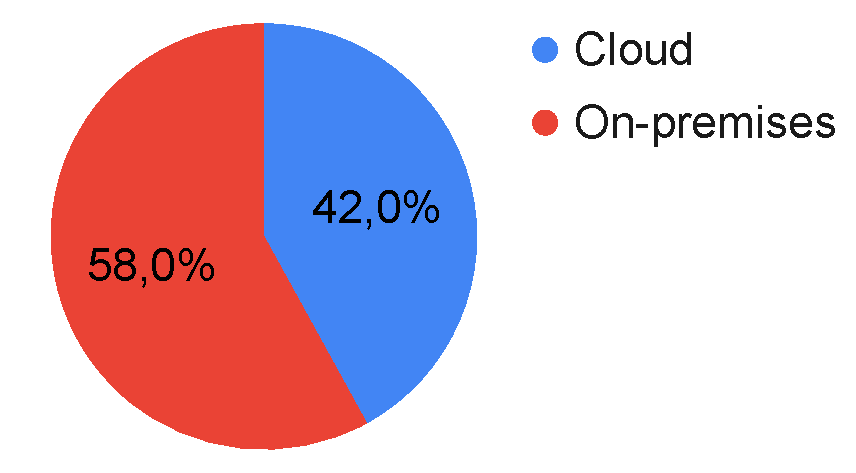
\epsfig{file = figs/re_cloud_on_prem.pdf, width = 5.0cm}}
  \caption{\textit{On-premises vs. cloud users.}}
  \label{fig:on_prem_vs_cloud}
\end{figure}

All on-premises clusters have one thing in common: They rely on the Hadoop ecosystem with YARN as a resource manager. In contrary, the participants working with cloud infrastructure, above all, use Databricks platform, which includes an own resource manager, the Databricks Serverless.

In terms of cluster sizes, the participants working with on-premises solutions, have in general bigger clusters, i.e. clusters with more nodes. The cluster size above 50 nodes is completely absent for the cloud, whereas it makes 27\% for the on-premises clusters. 

Regarding solutions used to work interactively on previously stated infrastructure, three possibilities are taken into account. Firstly, solutions included in a 3rd party platform or service, e.g. Databricks or Amazon EMR. Secondly, custom solutions, e.g. self deployed Jupyter or Zeppelin notebooks. Finally, it is possible that a participant does not work with any interactive environment. As seen in fig. \ref{fig:interactive_env}, 75\% of all participants work with an interactive environment. The 42\% referring to a 3rd party solution belongs entirely to the cloud users, thus every participant relying on the cloud infrastructure uses an interactive environment. On the other hand, only 55\% of on-premises users work with an interactive component. 

\begin{figure}[!h]
  \centering
   {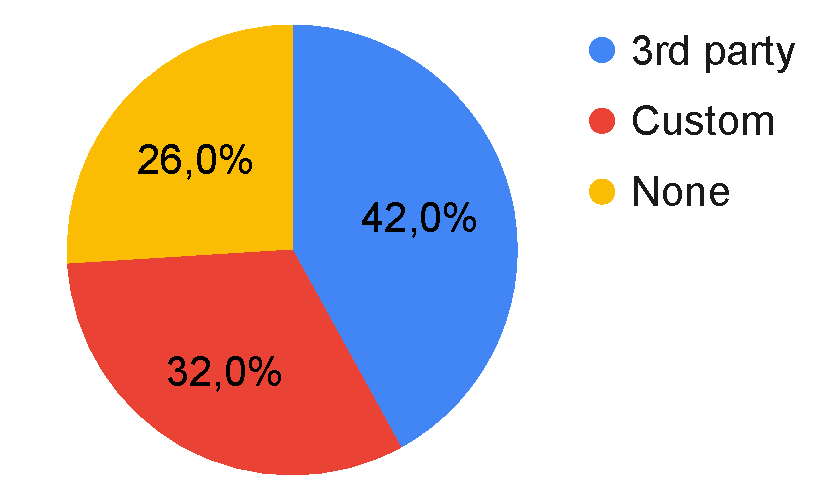
\epsfig{file = figs/re_interactive.pdf, width = 5.0cm}}
  \caption{\textit{Please specify, whether you use a custom made solution or a solution included in a third party platform / service for compute clusters.}}
  \label{fig:interactive_env}
\end{figure}

The fact that 45\% of on-premises users don’t work with any interactive environment encourages need for improvement, especially after deeper analysis of answers provided by
this group of users. 60\% of them finds features regarding interactive notebooks (which will be discussed further) important, which suggests, they are interested in working interactively.

Next, the actual setup used to work interactively is evaluated. A huge discrepancy between solutions utilized on on-premises and cloud infrastructure can be seen. Firstly, the platform of choice for cloud are notebooks included into the Databricks-Unified-Platform. It is used by 88\% of the participants working on cloud. The remaining 12\% belongs to Microsoft HDInsight, for which however, not much information has been provided, besides the average satisfaction score 3 out of 5. 

\subsubsection{Databricks}


In regards to Databricks-Notebooks, participants provide plenty of information. The major advantages named by the participants are the integration with other Databricks features, e.g. revision history and a tight integration with Microsoft Azure or Amazon AWS services, e.g. storage. Besides these positive aspects, 33\% of all Databricks users report poor flexibility or problems in terms of resource allocation for notebooks. As an extra commentary regarding this issue, one participant mentions the Databricks Serverless (resource manager). In his experience, the auto-scaling feature is very disappointing, since it does not dynamically scale the number of workers between specified minimum and maximum, but rather immediately increases to maximum even though the cluster usage is moderate. In addition, as he states, it never reduces the number of workers back once the workload on the cluster decreased. As this autoscaling feature of Databricks seems to be only working in one direction, users might be faced with increasing cost which could have been avoided. Another user complaints about memory allocation failures, which made him
switch from Databricks to local development (using R programming language). Further, Databricks is missing in terms of flexibility as it can be only used together with the cloud offered by Microsoft or Amazon and delivers limited customization possibilities. 

In spite of above negative aspects, one has to admit, in general, that Databricks is a powerful tool offering various different features and having tight Spark integration. Concluding from the achieved score during the requirements engineering process, it is a convenient and satisfying solution. On a scale 1 one 5, the average score Databricks has got is 3.85, which is a rather high rating. The highest given score was 4. In addition, this score confirms that for cloud there are indeed reliable products available, that allow to work with distributed data interactively. For on-premises, however, the situation is entirely different, as shown below. 

\subsubsection{Custom solutions}

Participants using on-premises infrastructure are working with \textit{custom} solutions. The word \textit{custom} has been used, since those solutions are not offered as part of a holistic platform or a service. They are configured and deployed manually by the cluster owner (or more likely, his employees). 50\% of said solutions consist of a manual deployment of Jupyter notebooks (or JupyterLab), the remaining 50\% include Zeppelin notebooks. 

Further, users were asked to describe their setting in a few words and provide advantages of it. Regarding description, the usage of a notebook requires connecting to the edge node
of the cluster via SSH through a terminal, and depending on the setup in place, spawning a notebook with a terminal command on said edge node or starting one from the Zeppelin UI. When using frameworks for distributed data processing like Apache Spark, one can conclude that the Spark Driver runs on the same machine as the notebook (or within the notebook). The only named advantage was the possibility of fast data exploration, e.g. with Spark SQL.

In terms of negative aspects or missing functionalities, plenty issues were provided. 50\% of users working with a custom solution complain about \textit{poor or none Spark integration with their interactive environment}. Furthermore, Zeppelin notebooks, as found during interviews, are very unstable and since the Spark Driver runs within the notebook, one has to kill the application manually if the notebook stops working. In result, a lot of restarts of Spark applications may be necessary.

\begin{figure*}[!h]
  \centering
   {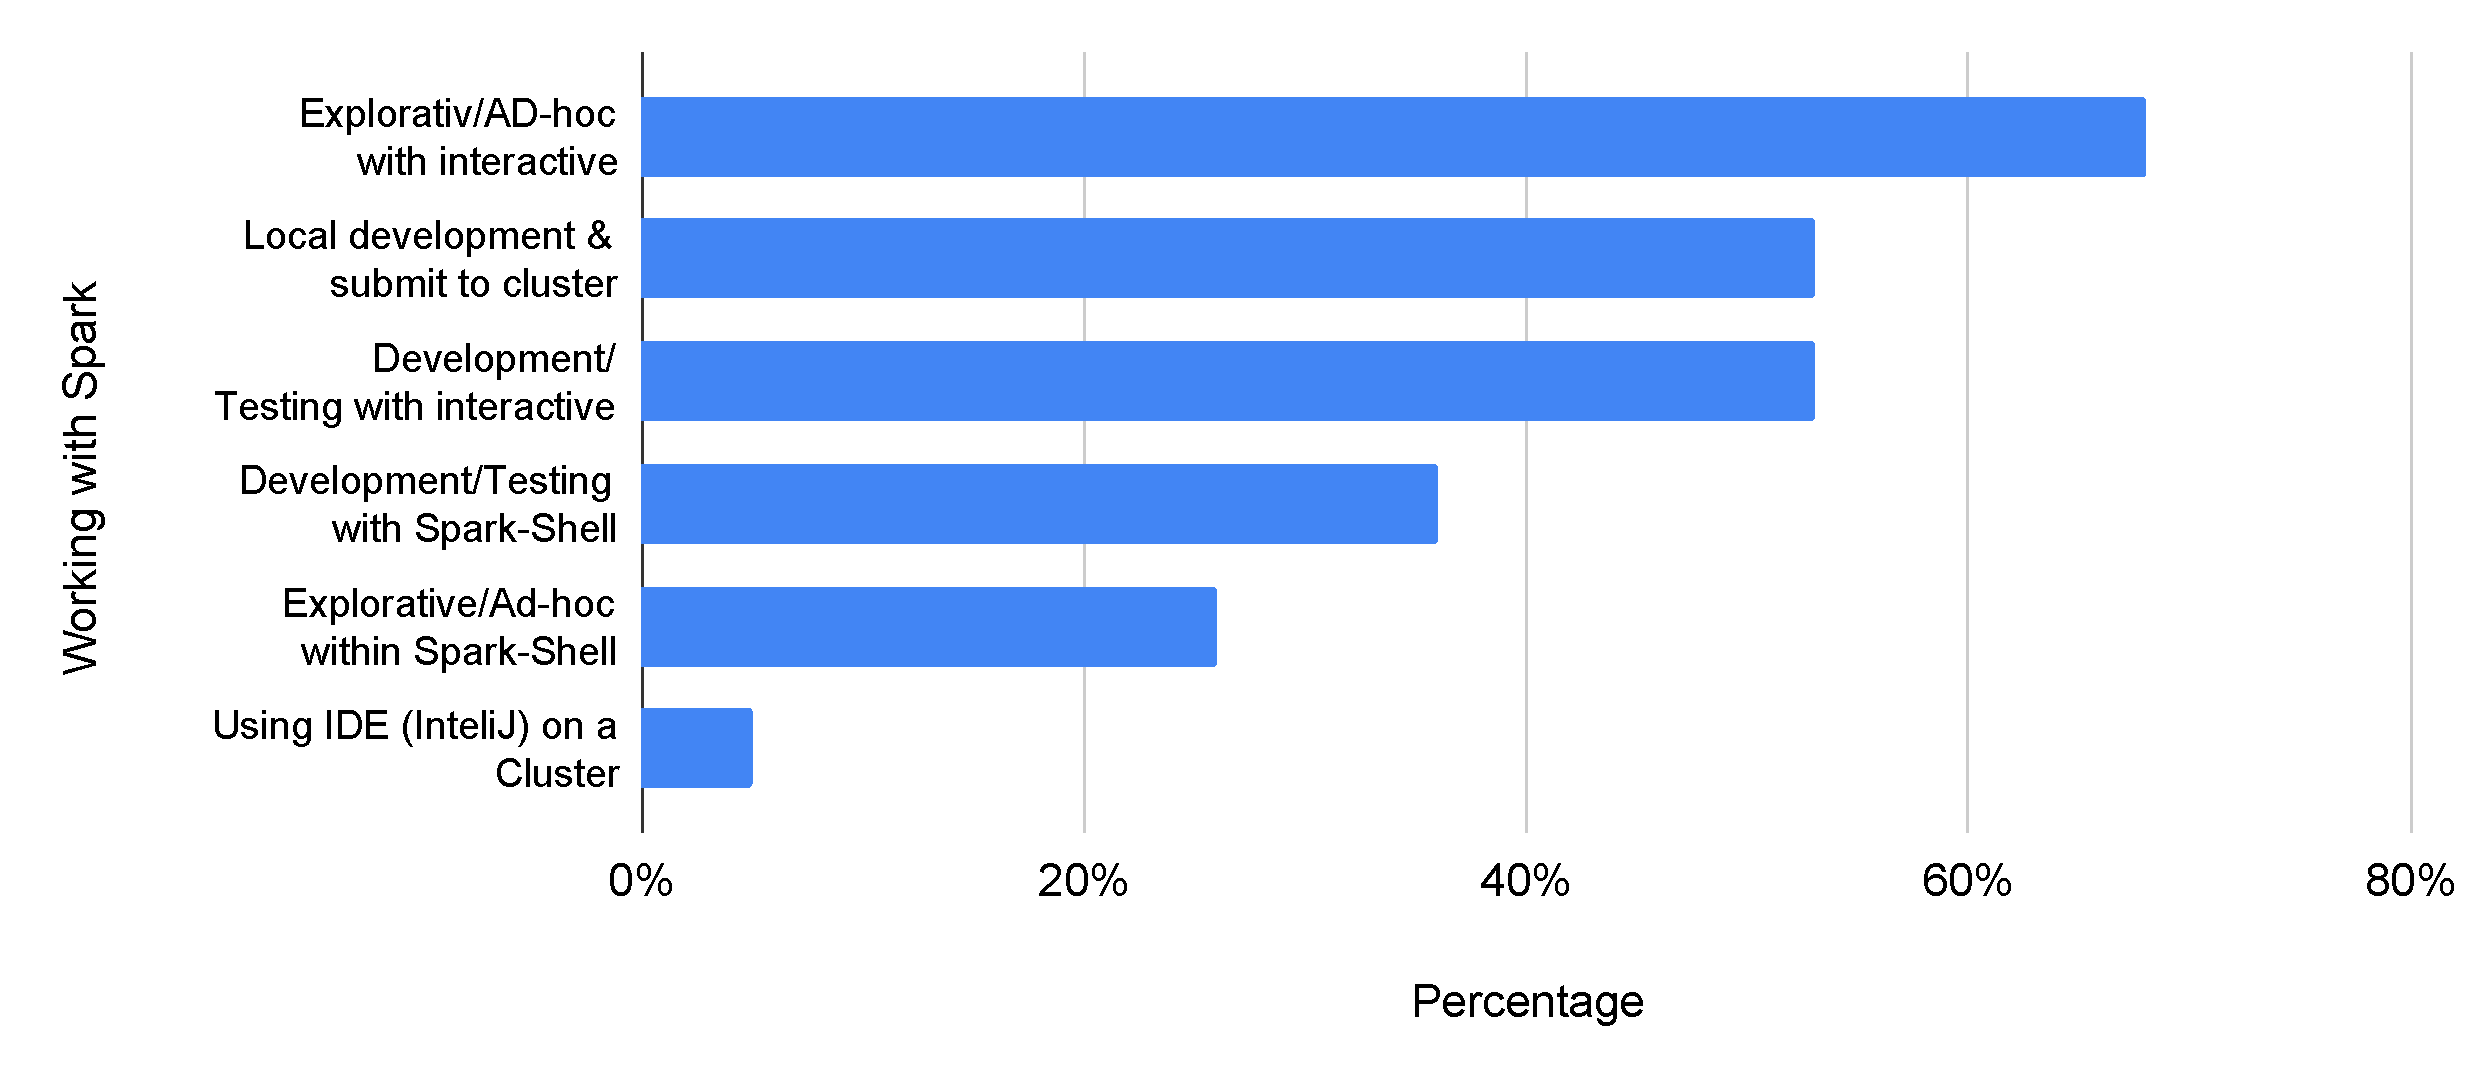
\epsfig{file = figs/re_how_spark.pdf, width = 14.0cm}}
  \caption{\textit{How do you mostly work with Spark on your cluster in terms of development and testing?} More than one answer was possible since one person can work with Spark differently, depending on the use-case.}
  \label{fig:re_how_spark}
\end{figure*}

Another common issue is \textit{poor user management}, criticized by around 50\% of participants.  \textit{Poor flexibility in terms of resource allocation for a notebook} is also a major issue. This has been especially discussed during the interviews. Since the notebooks run on the edge node (e.g. YARN master), the resources are quickly gone and the node is overloaded. The users have to manually keep track of which notebook (or Spark application) takes what resources. This manual tracking is done e.g. with a spreadsheet available for all users. Obviously this is not an optimal solution and it happens, that a user kills applications of another user to free resources. Also, since the notebooks are running on the edge node and Spark is executed in client-mode, it is possible to paralyze the whole edge node with one simple command. For example, if a user wants to collect a distributed dataframe back to the Spark driver, he can immediately utilize all available resources of the edge node. This issue and in general, the previously used architecture, are discussed more deeply in the \textit{Evaluation} section.

The lacking transparency of running applications inside the cluster was mentioned as well. Only the YARN UI is available, which, although very useful, is not quite user-friendly and a bit too technical for not experienced users. Another stated issue is \textit{poor flexibility in terms of notebook customization}.

In contrary to Databricks, provided drawbacks reflect in the average satisfaction score which is 2.67 out of 5. The highest given score was 3. Thus the situation with interactive data science and development is much worse for on-premises infrastructure than with cloud solutions.

\subsubsection{Framework for distributed data}

The question \textit{What frameworks for large amounts of distributed data do you use in your current setup?} provided strong and important realization, namely, every single participant uses mostly Apache Spark, despite other frameworks like e.g. Dask or Apache Flink being available on the market. Furthermore, 90\% of participants who use an interactive environment, utilize it together with Spark.

It is also important to know, how users actually work with Spark, especially to see how significant interactive notebooks are in context of Spark. Figure \ref{fig:re_how_spark} shows various ways to work with Spark sorted in descent order which corresponds to popularity among participants. As one can see, interactive environments are a big factor for working with Spark, especially for Ad-hoc data exploration, which is with 68\% the most frequently chosen option. Even development and testing of Spark applications with interactive notebooks is very popular, as it holds, with 53\%, the second place ex aequo with local development and submitting jobs to cluster. 

\subsubsection{Features}

The last part of the questionnaire and interview deals with features or functionalities that a platform of this kind should support. Participants were asked, how important certain features are and whether they are supported by participant's current setup. Here again, the differences between cloud and on-premises solutions are tremendous. While important features are mostly supported by cloud services or platforms, they are missing for most of the on-premises solutions.

The most important features, that are also mostly lacking for on-premises solutions (in descending order in terms of importance):

\begin{itemize}
    \item Specifying own resources for an interactive environment
    \item Transparent and easy accessible overview of allocated and free cluster resources
    \item Transparent and easy accessible overview of workloads running on the cluster
    \item Connecting to a Spark cluster from a local notebook session
    \item A UI from where a user can start notebook sessions
\end{itemize}

Based on gathered results, it is possible to specify requirements, a platform for interactive development with distributed data should fulfill. This is discussed in the following section.

\subsection{Resulting Requirements}

Due to the gathered information, it is possible to formulate requirements that a holistic platform for interactive data science on distributed data should fulfill. One of the key findings from the previous steps is the fact, that on-premises solutions are in general not
optimal and that YARN is the resource manager of choice for users working with their own compute clusters. Providing a full software requirements specification would be out of scope for this paper, thus a summary of the most important requirements follows. 

First of all, since the on-premises solutions are lacking in many aspects, it is important to support said infrastructure. Cloud solutions, although fairly advanced and well made, are restricted to be used only on selected clouds and are generally missing in terms of flexibility. Thus additionally, the platform should be deployable and usable on at least 3 major clouds: GCP, AWS and Azure.

The on-premises solutions analyzed during interview and questionnaire do not scale well. This should be improved. The architecture should support many users. Thus, utilization of all nodes should be
possible. The notebooks should not be deployed on the edge node but rather on all available nodes. In this case, the upper limit of users results from the cluster as a whole.


In a platform for interactive analytics on distributed data, the interactive component, i.e. a notebook, is essential. Hence it should be available. Furthermore, it is important to provide each notebook user with a personal storage for storing notebook files or smaller data sets. A shared storage containing large datasets, e.g. HDFS, needs to be accessible from a notebook as well. Such a platform should offer notebooks with frameworks like Apache Spark out-of-the-box, as Spark is the framework of choice for distributed data science. Furthermore, Spark should be available in cluster-mode, as to avoid previous bottleneck-problems that results from the client-mode.

In order to increase to user-friendliness and provide the user with useful functionalities, a Web-UI (user interface available from a browser), should be included into the platform. It should offer the possibility to create own interactive environments (with wished packages and resource specification). Further, viewing the cluster state and running applications should be offered by the Web-UI as well. Starting an interactive notebook from the UI should require not more than a few clicks. It is crucial, that as little as possible technical knowledge is required from a user, who wants to add an own environment and then start using it from within a notebook.

The possibility of adding own environments and specifying resources for it was especially deeply discussed during the interviews. While it is a desired and important feature, some participants think, users tend to allocate more than necessary. Thus, specifying own resources should be possible, but also subject to an administrative global limit. This functionality should also be included into the Web-UI, i.e. an administrator who can set limits in terms of resources for other users.

\begin{figure*}[!h]
  \centering
   {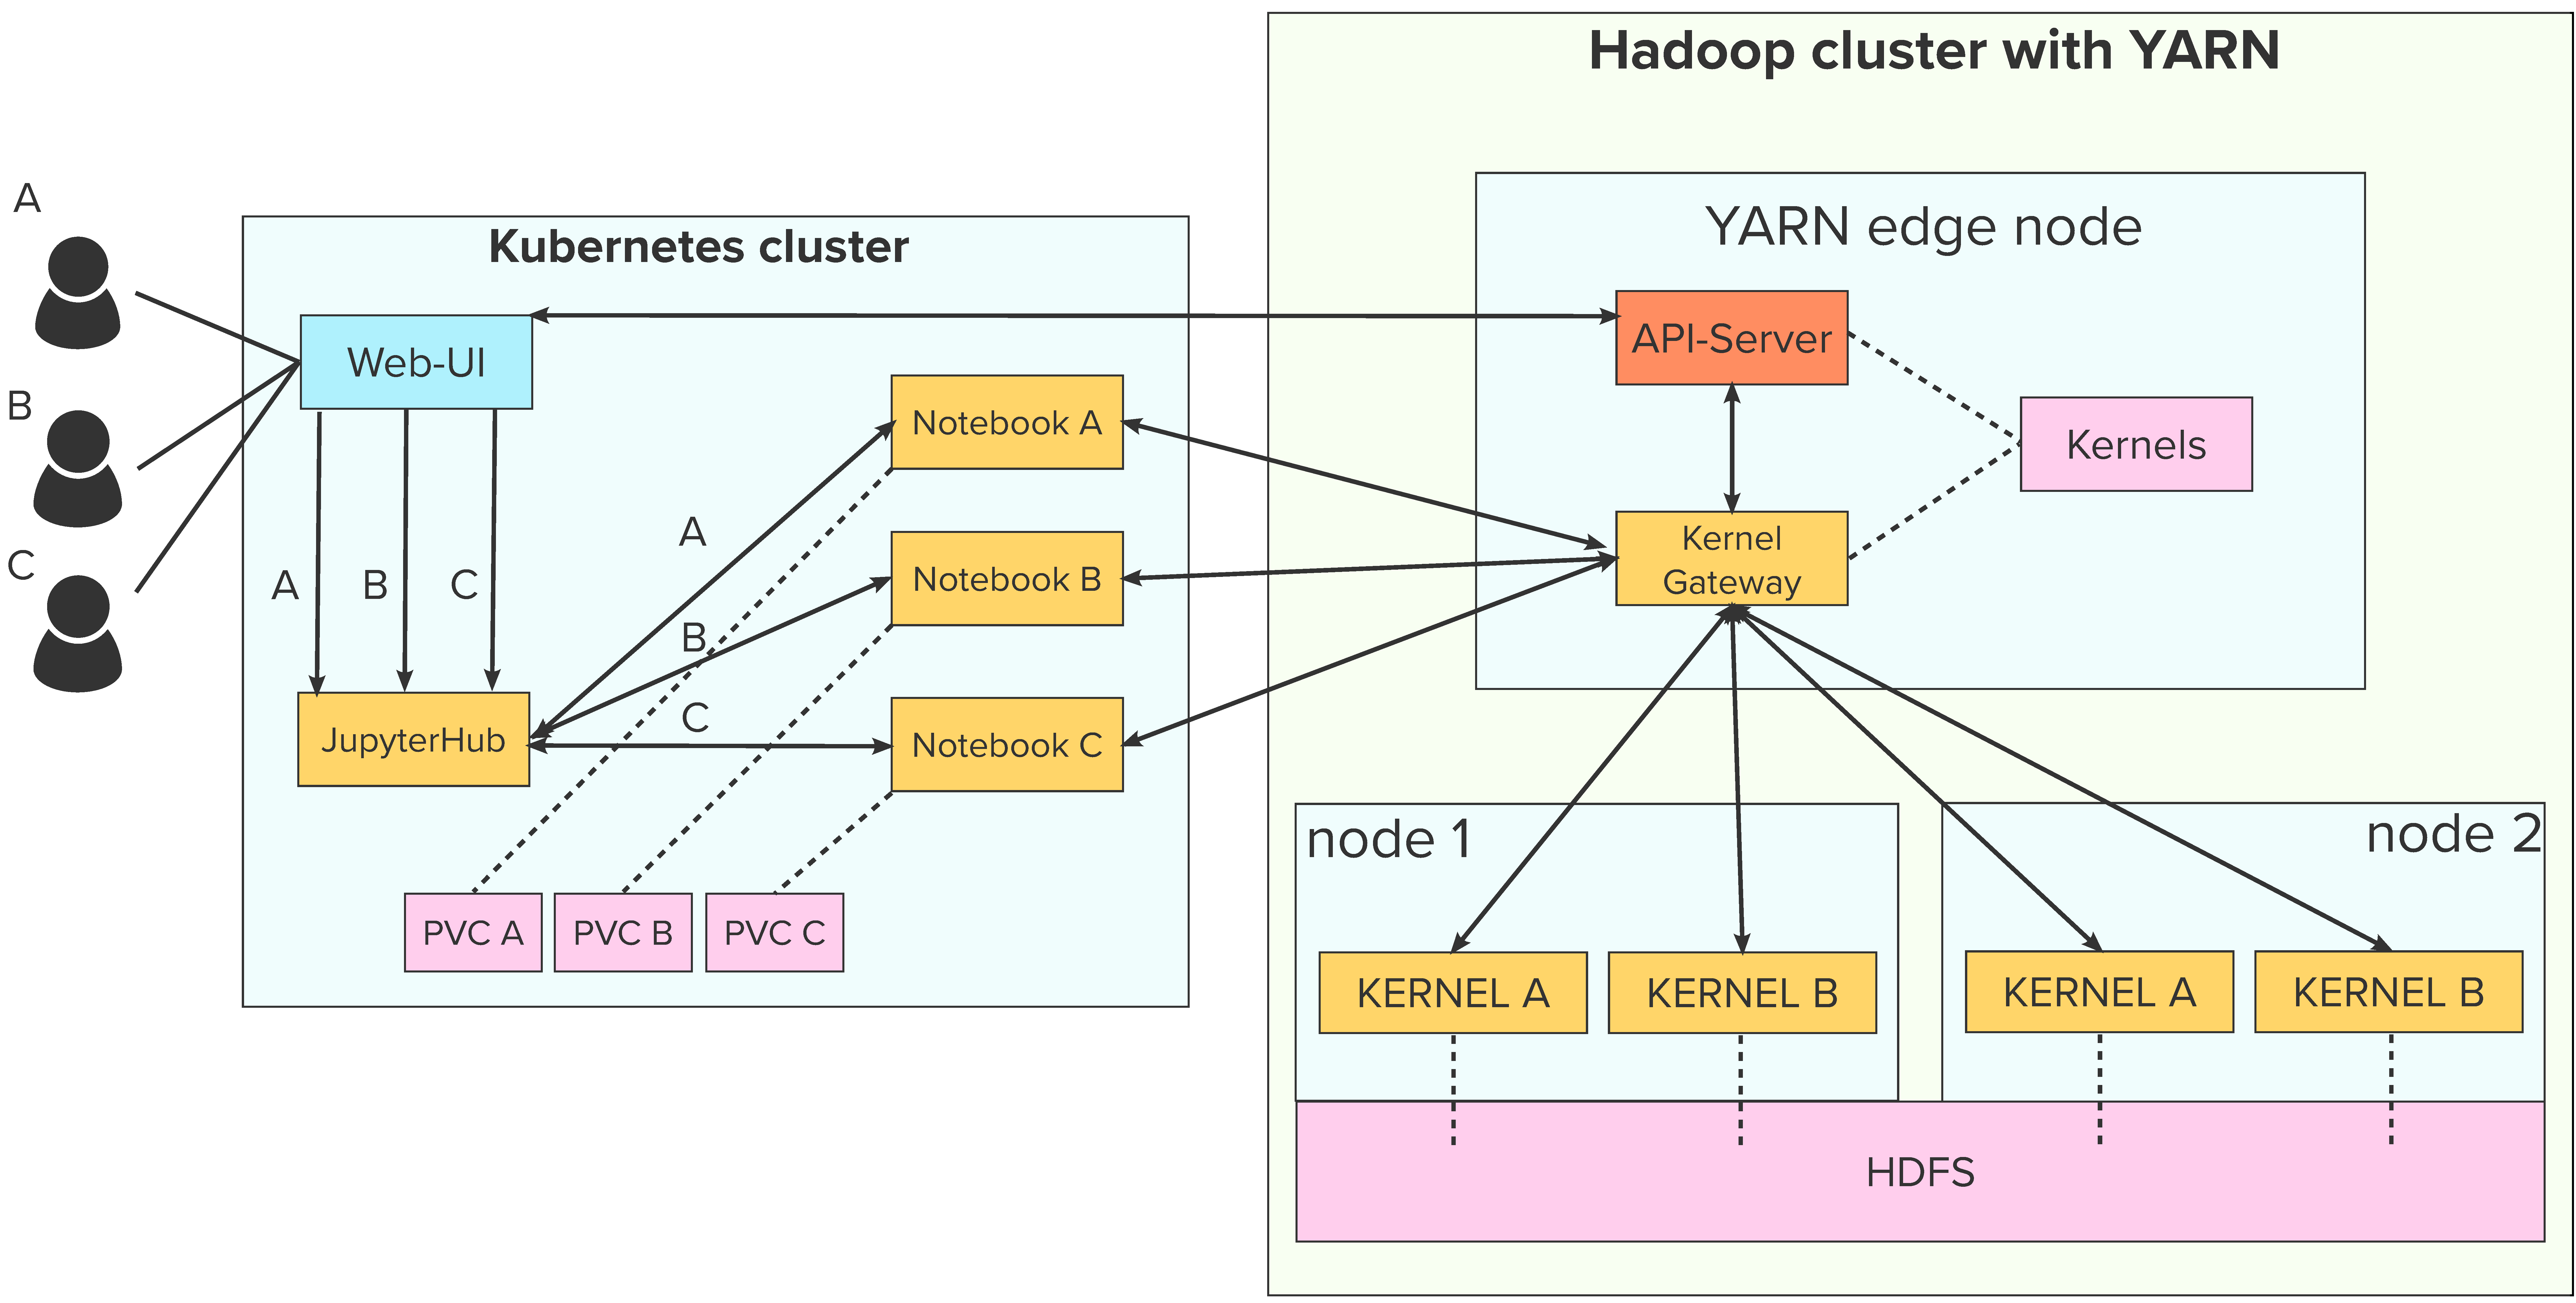
\epsfig{file = figs/concept_arch_kubernetes_yarn.pdf, width = 14.0cm}}
  \caption{Architecture based on both, YARN and Kubernetes. Ease of distributing notebooks and using YARN to manage the kernels combined.}
  \label{fig:kubernetes_yarn}
\end{figure*}

\section{\uppercase{Architecture}}

In order to satisfy previously stated requirements, a cross-cluster architecture is proposed.  As stated in in \textit{Requirements Engineering} section, every user working on an on-premises infrastructure relies on YARN. This is no surprise, since YARN is a mature system and has been used together with Spark for a long time. Hence supporting YARN together with Hadoop is necessary. However, running notebooks as managed resources leveraging underlying resource manager is quite challenging on a Hadoop cluster. In result, notebooks are spawned only on the edge node, which dramatically decreases the scalability. This is one of the issues, that solutions discovered during requirements engineering suffered from. 

The problem described above does not exist on a Kubernetes cluster. Kubernetes was designed to deploy and manage containerized applications. In this field, it offers many advantages. The deployment is easy to automatize and, above all, is clear in a sense, that it improves the overview of what is happening inside the cluster and allows
good control over the applications. Every container runs as a pod, which can be described in terms of resources in a fine-granular way. In result, every notebook runs as a container as well and is subject to Kubernetes' resource manager, i.e. notebook containers are distributed across the whole cluster, avoiding the bottleneck situation that occurs in a Hadoop cluster. 

Nevertheless, YARN still needs to be supported. Not only because of previously discussed requirements, but also because it offers a more dedicated resource manager, allowing e.g. queues. To combine these two worlds, Kubernetes and Hadoop, a kernel gateway is included into the platform. It separates the kernel (interpreter) from a notebook container. The notebooks still run on the Kubernetes cluster and are equally distributed across all nodes, their kernels however, run as manageable resource within the YARN clusters. 

A cross-cluster solution offers advantages of Kubernetes and YARN architectures. On the one hand, the deployment on Kubernetes site is much easier and more fine-granular, especially in terms of notebooks. As a notebook hub, JupyterHub is used. It supports Kubernetes deployment and offers distribution of single server notebooks across the cluster without much effort. On the other hand, the kernels are running in the YARN cluster, which means the advantages of Hadoop's resource manager can be utilized and the requirement for YARN support is fulfilled. 

The proposed architecture is presented in figure \ref{fig:kubernetes_yarn}. As one can see, the Web-UI is the entry point of the whole platform from where a user, redirected to the notebook hub, can start a notebook. Further, it offers the possibility to add own interactive environments by specifying desired programming language, additional packages and resources. Since the environment is strictly connected with a Spark kernel, the resource specification is typical to the one of a Spark application. Additionally, the Web-UI offers an easy to grasp overview of the YARN cluster, with the possibility to e.g. view logs of running applications. An admin view for restricting user actions in terms of resources is included as well. 

Once redirected to JupyterHub, a user can start an own interactive session in form of a notebook (JupyterLab). While creating a notebook container for a new user, a PVC (Persistent Volume Claim) is created, which offers access to storage of predefined size for each user. This private storage survives deleting a running notebook container and is available for the user after starting his notebook again. The usage of a PVC offers a good encapsulation against other users.

Each notebook spawned within the Kubernetes cluster is connected to the kernel gateway which runs within the Hadoop cluster. As kernel gateway the Jupyter Enterprise Gateway is used. It starts kernels on behalf of a notebook user. In this way, a separation between view (Kubernetes) and compute (YARN) logic is achieved. Further, since the kernel is separated from the actual notebook, utilizing Spark in cluster-mode from within a notebook is possible. Without the kernel gateway component, the kernel resides within the notebook container and thus Spark context lives within the client (notebook) and hence only client-mode is possible. This is a great improvement compared to all known solutions available for on-premises infrastructure. 

Each started kernel runs on one of the YARN worker nodes and has access to the HDFS. Thus a user using a notebook running within the Kubernetes cluster, can access a shared HDFS storage, where e.g. large datasets might reside. Hence both requirements, the personal and shared storage integration are satisfied.

In order to start a kernel, the kernel gateway needs to have access to kernel specifications. Each specification represents a complete interactive environment. Such environment can be added by a user from the Web-UI, as already mentioned. The kernel specifications are stored in a \textit{Kernels} directory visible in the above figure. 

For some functionalities of the Web-UI a built-in API-server from the resource manager or the kernel gateway can be used. For example, the cluster overview should deliver information about what's currently happening inside the cluster as well as about resource utilization. Most of these information can be obtained from the API of the resource manager. Similarly, a list of currently available kernels should be provided by the API of Jupyter Enterprise Gateway. Those APIs, however, do not cover all the necessary cases. Thus a custom API-server is needed. 

One major functionality that the API-Server should offer, is creating new kernel specifications, i.e. new environments for a user to work with. After a user has provided necessary parameters for a new kernel through the Web-UI, a request to the API-server should be sent, which in turn creates all the necessary files (in a place accessible for the kernel gateway, i.e. \textit{Kernels} directory), and send confirmation back to the Web-UI. Modifying available kernels should be handled similarly. Other functionalities are e.g. modifying Jupyter Enterprise Gateway configuration file, for example to change the number of allowed kernels run by one user or getting detailed information about kernels.

\section{\uppercase{Evaluation}}

The proposed architecture was realised as a proof-of-concept prototype. The technical requirements, e.g. Spark in cluster-mode from withink a notebook or scalability, were in foreground. However, the design of user-interfaces plays a big role as well, since the platform should ease the life of a data scientists and thus needs to be user-friendly. Thus various evaluation approaches has been taken. Firstly, a discussion about fulfilling stated requirements is given. Then, in order to prove high user-friendliness, a usability evaluation is given. Finally, since the platform should outperform previously used solutions, a brief comparison to a solution described by participants during requirements engineering takes place.

\subsection{Fulfilment of the specified requirements}

One of the crucial requirements is to support on-premises, but also cloud infrastructures. If it is possible to install YARN and Kubernetes,
any given infrastructure, whether on-premises or cloud, is suitable. Since GCP, AWS and Azure offer both Kubernetes and Hadoop services, all three clouds are supported. 

Further, the only components running on the YARN edge node are the ones that do not require to be scaled. The notebooks launched in Kubernetes are running as pods and thus are scheduled on the Kubernetes nodes evenly. The kernels of said notebooks are subject to the YARN resource manager and hence are distributed accordingly through the worker nodes. In this case, no bottleneck node is given and a larger architecture (more nodes) results in bigger upper limit for the amount of users or more resources for single users to be used. Thus high scalability is given. 

In terms of notebooks, on the one hand, the storage aspects, i.e. personal storage and shared storage accessible from within a notebook were already discussed in the \textit{Architecture} section. Both are given and thus said requirements are satisfied. On the other hand, Spark in cluster-mode is available from within a notebook due to the kernel gateway. 

Further, functionalities likes adding own interactive environments (with resource specification), viewing cluster state or setting limits for users are all included into the Web-UI. Hence these requirements are too fulfilled.

\subsection{User-Evaluation}

The user evaluation is meant to put the platform under stress. It is important to see, whether provided functionalities are usable in a user-friendly manner. Six tasks were prepared for each user. Furthermore, at the end, a user was asked 8 questions of a general nature. These questions come from the short version of User Experience Questionnaire (UEQ) and allow comparison to another software products \cite{schrepp2014applying}.

In total, 20 participants contributed to this evaluation.  Almost every participant has a background related to computer science and 60\% of them has a data science experience score 3 or higher out of 5. The average value is 3.05. Further, experience in terms of using notebooks was asked. The average score for the target group is 2.95, and 65\% has a score 3 or higher. Finally, experience regarding general usage of software was asked, resulting in an average score of 4.8.

Firstly, a user was asked to solve six tasks that refer to major functionalities of the platform. Each tasks was followed with questions regarding easiness and user-friendliness. Answers were possible within a range from 1 to 5, where 5 is the best score. The six tasks are presented below together with the average scores they have achieved:
\begin{itemize}
    \item \textbf{Kernel overview}: this task was meant to find out, how do users cope with the way the available kernels are presented. Participants were asked to tell how many kernels are available, find a kernel that has a specific package (pandas) installed and modify its resources. Easiness: 4.85, user-friendliness: 4.75.
    \item \textbf{Cluster overview}: in this task the users were asked to describe the current state of the (YARN) cluster in the \textit{cluster overview} page of the Web-UI. Easiness: 4.3, user-friendliness: 4.2.  
    \item \textbf{Adding a new kernel}: participants were asked to create a new kernel (new interactive environment) with provided specification. Easiness: 4.95, user-friendliness: 4.6. 
    \item \textbf{Using Jupyter notebook with created kernel}: in the previous task participants were asked to create an own kernel. In this one, they should use it from JupyterLab (requires starting a notebook from the Web-UI). Easiness: 4.65, user-friendliness: 4.75.
    \item \textbf{Using Jupyter notebook with created kernel}: in this task participants were asked to  view logs of their running notebook and kill it short after. A remark was added that this happens from the Web-UI and not from the JupyterLab opened in last task. Easiness: 4.1, user-friendliness: 4.6.
    \item \textbf{Managing limitations for users as administrator}: The last task required logging out and logging in as an administrator in order to set specified limits for users. Easiness: 4.55, user-friendliness: 4.6.
\end{itemize}

As shown above, the general user-friendliness of the platform is very high. One of the reasons for it, is the simplicity of provided functionalities and the fact, that there are only a few core functionalities. The named issues are mostly of rather aesthetic nature and the high score prove that the actual functionalities are present and well implemented.

This high score is also reflected in the UEQ benchmark. After completing these 6 tasks, each participant was asked questions from the short version of the UEQ template. The 8 items come with a 7 point answer scale. The resulting questions are based on said items, which are presented in \ref{fig:eva_ueq_general}. E.g. the first question is: \textit{How supportive do you find this platform?} The left side of the scale has a negative meaning, e.g. \textit{obstructive} and the right a positive, e.g. \textit{supportive}. Thus the middle of the scale results in a neutral answer and as a result, a scale from -3, through 0, to +3 is given.

\begin{figure}[!h]
  \centering
   {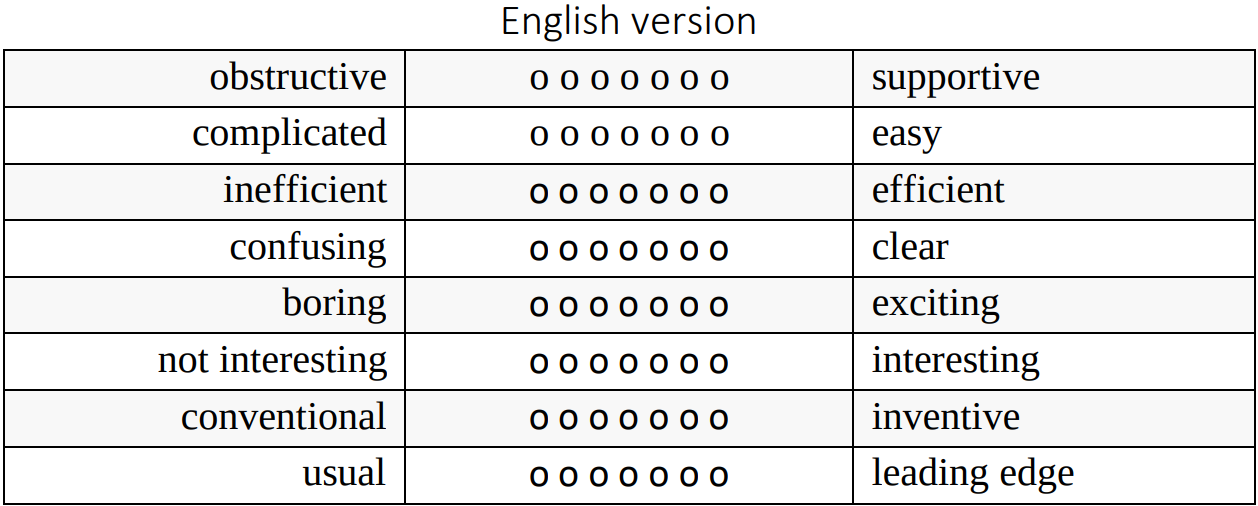
\epsfig{file = figs/eva_ueq_general.png, width = 7.5cm}}
  \caption{The 8 items of the short UEQ template. Each of these items were encapsulated in a question the participant was supposed to answer.}
  \label{fig:eva_ueq_general}
\end{figure}

The UEQ provides additional an Excel sheet where one can insert gathered results and a score consisting of three major qualities is generated from said 8 questions. Firstly, the pragmatic quality, i.e. usefulness, efficiency and ease of use. The second one is the hedonic quality, e.g. whether presented functionalities are original, interesting, engaging or exciting. Finally, an overall quality is given. Further, these qualities are shown in comparison to other software products, i.e. to data provided by 14056 persons from 280 studies. This benchmark is based on the full UEQ, thus using it together with short UEQ version should provide a reasonable approximation as stated in the mentioned Excel sheet. The resulting qualities can be seen in fig. \ref{fig:eva_ueg}. As one can see, the platform achieved a very high score and placed itself in the \textit{excellent} class. Below results for every item are briefly discussed.

\begin{figure}[!h]
  \centering
   {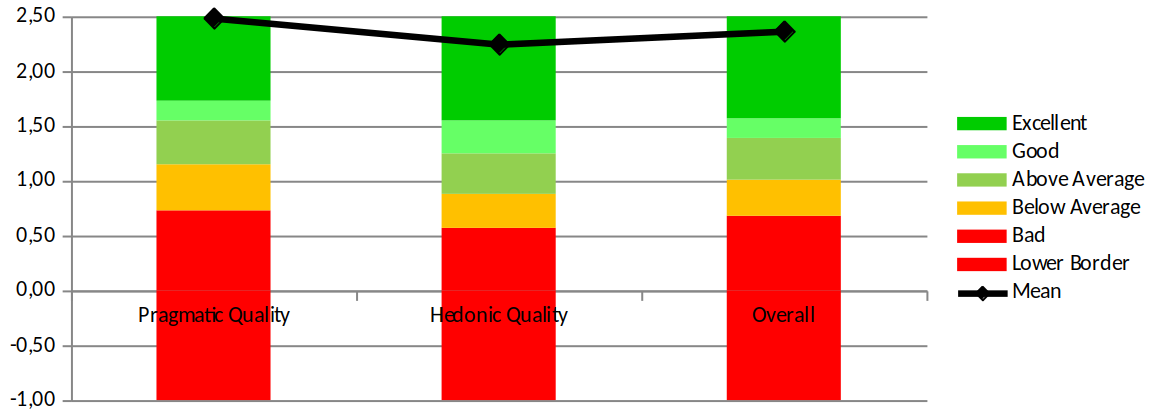
\epsfig{file = figs/eva_final_score.png, width = 7.5cm}}
  \caption{The benchmark provided by the UEQ template. A very high score was achieved.}
  \label{fig:eva_ueg}
\end{figure}

Referring to the scale from -3 to +3, for the first item, whether the participant finds the platform supporting, an average score of 2.6 is given. This high score can be explained by the simple fact, that creating Spark kernels and the general way to a notebook is very easy. Even users with lacking experience in data science and Jupyter notebooks can easily create a Spark kernel with wished libraries within a few minutes. They don't even have to specify resources since default ones are suggested. 

Further, as shown in previously, the general user-friendliness is very high and every task was rather easy to solve, hence the next three items, \textit{complicated - easy},  \textit{inefficient - efficient}, \textit{confusing - clear}, have got high scores as well, accordingly, 2.6, 2.6 and 2.2. 

The weakest item is the \textit{boring - exciting} item, which is part of the hedonic quality. Its average score is 1.8, which still is a good result. Although such a platform per se is not meant to be exciting, as stated by users, the architecture and things happening inside the platform are exciting to them. Further, other users were reluctant to describe the platform as boring. The item \textit{not interesting/interesting} has an average score of 2.8 which is caused by the fact, that single functionalities offered by the platform are interesting, e.g. adding own Spark kernels or the simple way to use notebooks. More technical users found the architecture very interesting.

Finally, the \textit{conventional - inventive} and \textit{usual - leading edge} items have got a score 2.4 and 2.1 accordingly. Some users were not familiar with data science platforms, hence for them it was something never seen before. Other users with better knowledge knew that similar platforms exist, however, not for on-premises infrastructures and not with Spark in cluster-mode from within a notebook, hence for them it was something new as well.

As discussed above, the users took into account not only the bare user interfaces, but also the actual functionalities that said UIs represent. Hence the presented score is not only about aesthetic of the platform, but rather about the advantages it brings, e.g. quick way to a Spark notebook or the \textit{cluster overview} that offers a rapid information about its current state. In terms of aesthetic, simplicity played a major role. E.g. in adding new kernel, only simple information need to be provided. The user interfaces was generally kept in a minimalistic style. These all are the reasons for the good results.

\subsection{Comparison against previous architecture}

During the conduction of requirements elicitation, users were asked to describe their current setup they use to work with Spark (interactively). Especially the interviews offered a chance to discuss this more deeply, above all, with the participants working with on-premises infrastructures. As a result, an architecture used by said participants can be presented and compared to the one conceived as a part of this paper.

In the previous solution, in order to start a notebook, a user needs to connect via SSH with the edge node. From there a manual start of a notebook is necessary (via terminal). While starting the notebook, the terminal command needs to contain resource specification, e.g. executor memory or number of executors. The kernel of said notebook runs within the notebook, i.e. Spark driver is the notebook itself. Thus Spark in client-mode is given. The kernel starts Spark workers that are distributed across the cluster. Since the notebooks with their kernel can only run on the edge node, a bottle neck is given leading to a quick overload of the edge node.

Further, since the notebook itself is not strictly restricted with resource limitations, if a user tries to put a distributed Spark data frame together, e.g by converting it to a \textit{Pandas} data frame, all data from executors will be taken back to the notebook, i.e. to the edge node. The kernel running within the notebook may growth out of bonds, crashing the whole edge node and disturbing other users.

This look entirely different on the platform proposed in this paper. While in the previous architecture everything has to be done manually via a terminal, the platform of this thesis offers a Web-UI, which provides useful functionalities and to start a notebook, one or two clicks are enough. Further, specifying resources for kernels in the previous architecture requires a lot of technical knowledge, since appropriate parameters need to be set manually, e.g.  \textit{--executor-memory=1024M} should be included in the notebook starting command. While users with technical knowledge should not have bigger problems with it, less experienced users may be overwhelmed. With the Web-UI, setting parameters is not necessary, only providing values or taking default ones.

Further, since the notebooks are not deployed on one specific node, but rather are subject to Kubernetes' resource manager, the scalabiltiy is tremendously improved and no bottleneck is given. In addition, the problem with putting a distributed Spark data frame has less negative influence. Since Spark in cluster-mode is given, the Spark Driver is not bound to client (notebook), but is subject to resource manager (YARN). Thus if such scenario should happen, the kernel application will simply run out of resources and fail, not distributing other users. Furthermore, Spark in cluster-mode allows much better and fine-grained distribution, since smaller components are present and thus scalability factor is increased.



\section{\uppercase{Conclusion}}

\begin{itemize}
    \item As next, a better user-management 
    \item As, next, collaboration aspects
    \item A short discussion about extending the functionalities to manage multiple Hadoop clusters from Kubernetes
\end{itemize}

\begin{itemize}
    \item Specified requirements result in a proof-of-concept solution
    \item The requirements are highly satisfied
    \item The evaluation yields very good results in terms of user-friendliness
    \item 
\end{itemize}


\bibliographystyle{apalike}
{\small
\bibliography{example}}

\end{document}

